\documentclass[]{article}
\usepackage[spanish]{babel}
\usepackage{listings}
\usepackage{xcolor}
\usepackage{graphicx}
\definecolor{codegreen}{rgb}{0,0.6,0}
\definecolor{codegray}{rgb}{0.5,0.5,0.5}
\definecolor{codepurple}{rgb}{0.58,0,0.82}
\definecolor{blackcolor}{rgb}{0.95,0.95,0.92}
\lstdefinestyle{mystyle}{
backgroundcolor=\color{blackcolor},
commentstyle=\color{codegreen},
keywords=\color{magenta},
numberstyle=\tiny\color{codegray},
stringstyle=\color{codepurple},
basicstyle=\ttfamily\footnotesize,
}

%opening
\title{Trabajo Final HCC}
\author{Nicolas Mendoza,  
María del Rosario Biangardi}

\begin{document}

\maketitle


\section{Introducción}
{\small {\normalsize En el presente trabajo se realizó la confección de un código para caclular y graficar la capacidad de sorción en el equilibrio (qe) a partir del ingreso de una tabla de datos experimentales de ensayos de adsorción de cinética y equilibrio en medio liquido . Las tablas ingresadas requieren tener las siguientes variables: para ensayo de cinética valores de concentración inicial (Ci), concentración en el equilibrio (Ce), tiempo (t), volumnen (V) y masa (m). Para el ensayo de equilibrio la tabla requiere de valores de concentración inicial (Ci), concentración en el equilibrio (Ce), volumnen (V) y masa (m).
		
		El programa calcula los promedios de cada variable, realiza estadística descriptiva y grafica los datos experimentales. Por otra parte, compara los datos experimentales con modelos teóricos y elige el modelo al que mejor ajusta.  
		 }}
\section{Herramientas computacionales utilizadas}
El programa se realizó en el lenguaje python, se trata de dos scripts:
 uno para el analisis de los datos de cinética y el otro para los datos de isotermas de adsorción. Cada uno de estos consta de un archivo principal y otro de funciones. El programa principal incia con la importación de la librería \textit{pandas}
\begin{lstlisting}[language=Python,style=mystyle]
 import pandas as pd
 \end{lstlisting}
 
 Siguiendo con la descripción del programa principal, el mismo consta de cinco partes, en la primera parte se define el archivo, y luego se lee como un dataFrame.
 \begin{lstlisting}[language=Python,style=mystyle]
 	archivo = "datosaleer.txt"
 	df = pd.read_csv(archivo, sep="\t", decimal= ",")
 	print ("datosaleer\n")
 	print (df)
 		
 \end{lstlisting}
 
  La siguente secuencia se invocan a una serie de funciones desarrolladas en el código secundario
  
  \begin{lstlisting}[language=Python,style=mystyle]
  	
  	df_promedio = promediar_y_calcular_qe(df)
  	estadistica_descriptiva= estad_por_grupos (df)
  	grafico= grafico_qe_vs_t()
  	grafica_ajustes = ajustes_resultados ()
  	
  \end{lstlisting} 
  
   Para el programa secundario, que contiene las funciones específicas, y es donde se encuentra el desarrollo del análisis,  se importan \textit{pandas, numpy, matplotlib, sklearn }
  \begin{lstlisting}[language=Python,style=mystyle]
  	import numpy as np
  	import matplotlib.pyplot as plt
  	import pandas as pd
  	from sklearn.metrics import r2_score
  	from scipy.optimize import curve_fit
  	from scipy.stats import t
  	
  \end{lstlisting}
  
  La primer función promedia los valores de los datos triplicados, agrupando por tiempo para el caso del ensayo de cinética y por concentración inicial para los ensayos de isotermas. La variable volumen [V], siempre es un valor constante. Luego calcula el qe para cada valor promediado y grafica los datos experimentales.
  
  
  
  
 Ejemplo para el ensayo de cinética:
 \begin{lstlisting}[language=Python,style=mystyle]	
 def promediar_y_calcular_qe(df):
 	global promedios
 	promedios = df.groupby('t', as_index=False)
 	[['Ci', 'Ce','m']].mean()
 	
 	# Tomar V correspondientes al primer valor por tiempo
 	vm = df.groupby('t', as_index=False)[['V']].first()
 	
 	# Unir ambos dataframes
 	global df_promedio
 	df_promedio = pd.merge(promedios, vm, on='t') 
 	
 	# Calcular qe
 	df_promedio['qe'] = (df_promedio['Ci'] - df_promedio['Ce'])
 	 * df_promedio['V'] / df_promedio['m']
 	
 	# Calcular qe individual para desviaciones
 	df['qdsv'] = (df['Ci'] - df['Ce']) * df['V'] / df['m']
 
 	# Mostrar el resultado final
 	print("\nDatos promediados y qe calculado:")
 	print(df_promedio)
 	
 \end{lstlisting} 
 
 La segunda función se encarga de realizar los cálculos correspondientes a la media, el desvío estándar y margen de error.
 
 \begin{lstlisting}[language=Python,style=mystyle]
 def estad_por_grupos(df):    
   global stats_df
   stats_df = df.groupby('t').agg(
   media_qe=('qdsv', 'mean'),
   std_qe=('qdsv', 'std'),
   n=('qdsv', 'count')).reset_index()
   
   stats_df['error-st'] = stats_df['std_qe'] / np.sqrt(stats_df['n'])  # error estándar
   stats_df['marg-error'] = stats_df['error-st'] * t.ppf(0.95, stats_df['n'])  # intervalo de confianza 95%
   
   print("\nEstadísticas por grupo:")
   print(stats_df)
 \end{lstlisting} 
 
 La tercer función grafica los datos experimentales de qe en función del tiempo para los ensayos de cinética y qe en función de la concentración en equilibrio para los ensayos de equilibrio.
 En primer lugar se definen las variables a graficar, se llama la función plot, se designan las variables dentro del gráfico y la mejor curva de ajuste estadístico. Por último, se detallan los lebels necesarios para  la mejor visulización y se observa el resulatado.
 Aquí se muestra una sección de la función encargada de graficarpara el ensayo de cinética:
 \begin{lstlisting}[language=Python,style=mystyle]
def grafico_qe_vs_t():
   x2 = df_promedio['t']
   y2 = df_promedio['qe']
   global yerr
   yerr = stats_df['marg-error']
 	
   plt.figure(figsize=(6, 4))
   plt.scatter(x2, y2, color='green', label='Cinetica experimental')
   plt.plot(x2_suave, mejor_modelo(x2_suave), ':', color='#88E788',
\underline{}   label=f'Ajuste grado {mejor_grado} (R² = {mejor_r2:.3f})')
   plt.show()
 	
 \end{lstlisting} 
 
 La última función determina el mejor modelo para los datos experimentales ajustados. Esta función dentro del programa de cinética considera tres modelos que son: pseudo primer orden, pseudo segundo orden y Elovich. Para el programa de isotermas los modelos considerados son: Langmuir, Freundlich y Temkin. Para todos los casos considerados los modelos fueron escritos como una función dependiente de las variables experiemntales ajustadas y los parámetros específicos de cada función.
 Ejemplo de modelos para los ensayos e cinética:
 
 \begin{lstlisting}[language=Python,style=mystyle]
 def ajustes_resultados():
    # Pseudo primer orden
    def pseudoPrimerOrden(t, qe, K1):
        return qe * (1 - np.exp(-K1 * t))
    
    # Pseudo segundo orden
    def pseudoSegundoOrden(t, qe, K2):
        return (qe**2 * K2 * t) / (1 + qe * K2 * t)
    
    # Elovich
    def elovich(t, a, b):
        return (1 / b) * np.log(1 + a * b * t)
    	
 \end{lstlisting} 
 Se realizan ajustes en función de los parámetros y los datos para poder extraer el coeficiente de determinación (r2). A continuación se muestra un ejemplo del código con la función de ajuste para el modelo de pseudo primer orden:
 
 \begin{lstlisting}[language=Python,style=mystyle]
 #PFO
   params_pfo, _ = curve_fit(pseudoPrimerOrden, t, qt, bounds=(0, np.inf))
   qe_fit_pfo, K1_fit = params_pfo
   qt_ajustado_pfo = pseudoPrimerOrden(t, qe_fit_pfo, K1_fit)
   r2_pfo = r2_score(qt, qt_ajustado_pfo)
 	
 	
 \end{lstlisting} 
 
\normalsize 
\section{Resultados}
\subsection{ensayos de cinética}

 \begin{center}
 \begin{lstlisting}[language=Python,style=mystyle]
 	    	
 	    t      Ci       Ce      m   V         qe
 	0   10  46.014  29.2955  21.85  20  15.302975
 	1   20  46.014  22.1740  21.40  20  22.280374
 	2   30  46.014  18.5690  21.45  20  25.589744
 	3   45  46.014  12.4825  22.80  20  29.413596
 	4   60  47.499  13.0815  21.05  20  32.700713
 	5   75  53.312  13.3050  21.25  20  37.653647
 	6  120  46.014   6.6530  21.95  20  35.864237
 	7  180  53.312   6.6730  21.30  20  43.792488
 	8  240  46.014   9.4850  20.35  20  35.900737
 \end{lstlisting}
\end{center} 
\begin{center}
	\caption{Tabla 1. Variables experimentales promediadas y calculadas}
\end{center}

 \begin{lstlisting}[language=Python,style=mystyle]
 		
 	Estadísticas por grupo:
 		t   media_qe    std_qe  n  error-st  marg-error
 	0   10  15.192375  5.257830  2  3.717847   10.856060
 	1   20  22.291466  1.678440  2  1.186836    3.465544
 	2   30  25.574667  3.048886  2  2.155888    6.295162
 	3   45  29.413596  0.345490  2  0.244298    0.713347
 	4   60  32.862217  4.578916  2  3.237783    9.454279
 	5   75  37.692558  4.677429  2  3.307442    9.657683
 	6  120  35.862410  1.134391  2  0.802136    2.342225
 	7  180  43.832513  4.018873  2  2.841772    8.297935
 	8  240  35.848428  4.301228  2  3.041428    8.880925
\end{lstlisting}
\end{center} 
\begin{center}
	\caption{Tabla 2. Estadísticas de los datos}
\end{center}
\begin{center}
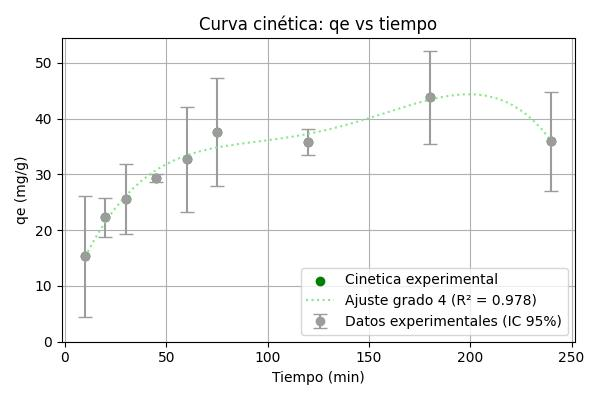
\includegraphics[width=0.8\linewidth]{imagenes/cinetica-1}	
\end{center}	
\begin{center}
	\caption{Figura 1. Datos experimentales y ajuste}
\end{center}
\begin{center}	
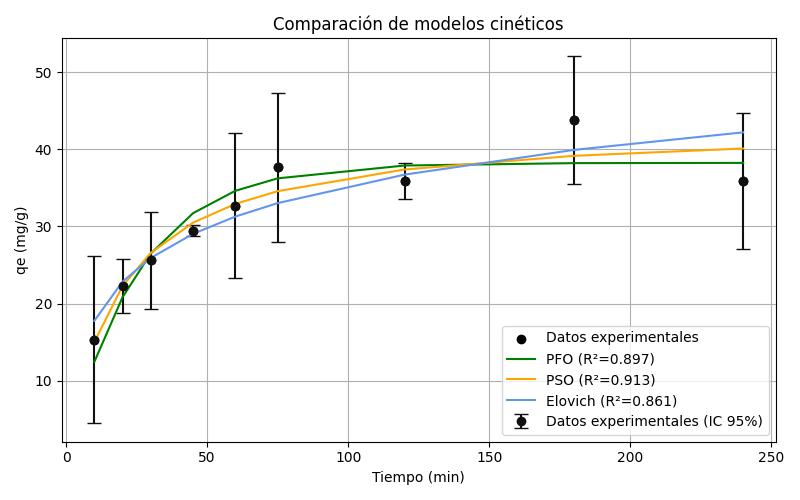
\includegraphics[width=0.8\linewidth]{imagenes/cinetica-2}
\end{center}
\begin{center}	\caption{Figura 2. Modelos ajustados}
\end{center}	

\section{Bibliografía}

Niaei, H. A; Rostamizadeh, M.(2020). Adsorption of metformin from an aqueous solution by Fe-ZSM-5 nano-adsorbent: Isotherm, kinetic and thermodynamic studies.The Journal of Chemical Thermodynamics, Volumen 142,106003.
https://doi.org/10.1016/j.jct.2019.106003.

\vspace{10pt}
Shahryari, Z.; Soltani, A.; Azadi, M. (2010). Experimental study of methylene blue adsorption from aqueous solutions onto carbon nano tubes. Int J Water Resour Environ Eng. 2.
\vspace{10pt}

Wang, J.; Guo, X. (2020). Adsorption isotherm models: Classification, physical meaning, application and solving method,Chemosphere,Volume 258, 127279. https://doi.org/10.1016/j.chemosphere.2020.127279. 

\end{document}
